\documentclass[a4paper,11pt]{article}

% ------------ Renew commands to have correct counting in enumerate env

\renewcommand{\theenumi}{\thesubsection.\arabic{enumi}}
\renewcommand{\labelenumii}{\theenumii}
\renewcommand{\theenumii}{\theenumi.\arabic{enumii}.}

% ------------ Import Requirements Elicitation for Referencing
\usepackage{xr}
\externaldocument{../Requirements/Requirements_Elicitation}

\usepackage[utf8]{inputenc}
\usepackage[top=3cm, bottom=3cm, left=3cm, right=3cm]{geometry}
\usepackage[none]{hyphenat}
\usepackage{xcolor,colortbl}
\definecolor{Gray}{rgb}{0.9,0.9,0.9}
\usepackage{graphicx}

% ------------ Title section
\title{
\vspace{-8cm}
\begin{flushleft}
    \vspace{10cm}
    \normalfont \normalsize
    %\Huge Bachelor/Master Thesis Project \\
    \vspace{-1.3cm}
\end{flushleft}
\vspace{3cm}
\begin{flushleft}
    \huge Face Recognition System \\
    \LARGE  Design Document\\
\end{flushleft}
\null
\vfill
\begin{minipage}{\textwidth}
\begin{flushleft} \large
\emph{Authors:} Walid Balegh, Jakob Heyder, Sarpreet Singh Buttar, Henry \hspace{45pt} Pap and Oscar Maris \\ % Author
%\emph{Supervisor:} Name of your supervisor\\ % Supervisor
%\emph{Examiner:} Dr.~Mark \textsc{Brown}\\ % Examiner (course manager)
\emph{Semester:} VT 2017\\ %
%\emph{Subject:} Computer Science\\ % Subject area
\end{flushleft}
\end{minipage}
}

\date{}

\begin{document}

\maketitle

\newpage

\tableofcontents

\newpage


\section{Introduction}
The FRS (Req. \ref{ReqDefinitions}) design document is intended to be the groundwork of how the software should be built. Members of the development team should be able to read this and have a similar understanding of how the software should be developed. Details of the known unknown will also be documented here.
%still working on the indroduction don't want it to sound too much like purpose

\subsection{Purpose}
The design documentation of the FRS is intended to create a mutual understanding of the software's functionality and contents. This document should contain all necessary information to start development of the face recognition system. This includes all known technologies, pitfalls and the architecture that are necessary to the FRS as a whole. 

\subsection{Definitions, acronyms and abbreviations}
\begin{itemize}
 
\item \textbf{FRS : Face Recognition System to be developed} (Req. \ref{ReqDefinitions})
\item \textbf{PN : Swedish Personal Number} (Req. \ref{ReqDefinitions})
\item \textbf{User-Entity: A User entity consists of an identifier(ID), a personal number and a link to a picture of the person} (Req. \ref{ReqDefinitions})
\end{itemize}
 
See Requirements document for related acronyms and references.

\subsection{References}

Requirements Elicitation v1.0 of the Face Recognition System for  LNU. Often mentioned as Requirement Elicitation, Requirements or "Req.", which a referenced chapter.


\subsection{Priorities}
%Priorities
%	- Security - Encryption and Authentication , sensible data
%	- Portability/Integration \& Usability - clear defined API
%	- Reliability

\textbf{Security}: As we are dealing with users private information it is imperative that the system is both secure and has limited access for both users and administrators. The primary methods to achieve this will be: The use of HTTPS SSL/TLS \ref{ReqConstraints}  and both admin and user authentication. \\ \\
\noindent
\textbf{Reliability}: When the user requests a PN from the server there needs to be a certain guarantee that that the PN returned matches the image provided. In order to accomplish this, the skybiometry api will have to meet a certain percent level of the two compared faces. The required percent level will be parameterized and on request can be defined and changed by the customer. \\ \\
\noindent
\textbf{Speed}: The primary function for the user side of the FRS, the GET request (Req. \ref{UAMRet}) is constrained to have a five second process time when returning a PN. (Req. \ref{ReqConstraints}) The relevance of this number is to ensure user friendliness to the client.
%in other words this was an arbitrary number set by the client to ruin our day
Since this relies heavily on the response time of the external API, this must be archived in cooperation with skybiometric. This does not effect further design decisions, since the requests for a single entity have to be handled synchronously and the process time is highly dependent on the production-deployment environment. Further handling and validation will be part of the testing phase for production deployment. 
\subsection{Overview}
This design document is for a face recognition software. The FRS purpose is to provide a PN (Req. \ref{ReqDefinitions}) using a comparison of a user provided image of a person's face. There should  be authentication to both users and administrators. Administrators should have access to a list of the PNs from the database. Administrators have the functionality of add, edit, list and delete user-entities from the database (Req. \ref{ARMFunctionality}).
Additionally to the FRS an example user application, known as the UAM (Req. \ref{ReqDefinitions}), will be developed to present the functionality of the systems API. Said application should include the ability to authenticate the user, request PNs using images and show the CRUD functionality of the administrator.

\newpage
\section{Major Design Issues} \label{Major_Design_Issues}
In this section all major design issues and decisions will be discussed. Rational and alternatives will be presented. The detail of evaluating the alternatives depends on the trade off the decision has.

\subsection{Architectural Design} \label{2.1 Architectural Design}
As desired from the customer the system will have a Client-Server structure. Where the in section \ref{ReqDefinitions} of the Requirements Elicitation defined UAM and AAM are the client modules and the URM and ARM are the server modules. Further we may reference URM or ARM as Server and UAM and AAM as Client. It is important to note that as defined in the requirements Req. Doc. \ref{ReqSystemInterfaces} our developed product is only the Server with a clear defined API and the Client application is the desired example client to show how integration and usage could be done.
The architecture of the server is defined in detail in Section \ref{Architecture}.

\subsection{Languages \& Frameworks}
In this section Technology's for the server concerning language and frameworks will be reasoned and concluded.
\subsubsection{Server-side}
As choice of programming language we choose the \textbf{Java programming language}. It is one of the most widely used ones on the server side. Especially the  in \ref{ReqProductFunctions} of the Requirements Elicitation defined REST functionality is supported by various frameworks with large communities. Rationals which led to the choice are listed below.
\begin{itemize}
\item Great flexibility \& portability due to platform independence with the JVM.
\item Scalable solution based on proven enterprise solutions
\item High productivity because of existing frameworks and solutions
\item Good support by a large community of developers
\end{itemize}
\noindent
The Spring Framework will be used on the server side of the system.
More detailed the Spring Web, Security, Data and Boot modules. 
The Spring Framework allows fast, enterprise scale development of applications by providing features for security, RESTful applications and Data Management and thus is the perfect fit for the requirements defined in the Requirements Elicitation \ref{ReqProductFunctions} and \ref{ReqConstraints} such as authentication, encryption and REST functionality. The Rationals for using the different modules are listed more detailed below.
\begin{itemize}
\item Great Portability and Integration - it is supported by various cloud providers to make deployment and continuous development possible.
\item Spring Boot provides an embedded application server which allows fast and easy setup of an application.
\item Configurability - Spring is easily set up and gives good default solutions but also provides the possibility to configure the details to the application needs
\item The Spring framework provides RESTful support which is asked for from the customer and fills the application needs.
\item Spring Data provides a convenient way to implement CRUD functionality for accessing and modifying data. It supports various Database technologies such as JPA and generates boilerplate code at run time which reduces developing costs.
\item Spring Security provides enterprise ready security features for authentication and encryption without much setup.
\end{itemize}

\subsection{External Services}
The external services needed to develop the FRS will be discussed and covered here. If there are multiple technologies that could be considered, they will be reasoned and selected within this section. 

\subsubsection{External Face Recognition API}
One of the core features as defined in \ref{ReqProductFunctions} of the Requirements Elicitation is to match a photo of a face with an existing one to a certain factor of equivalence/similarity. For this purpose as defined in the requirements an external service will be used. Following we compare some of the most known ones. Important aspects are cost factor, usability for the specific needs and security support.
There are some External Face Recognition API out there such as
\begin{itemize}
\item \emph{SkyBiometry: } It is a cloud-based face detection and recognition software which provides a high-precision biometric identification for over 20 years. In addition, it also provide API client libraries in various languages such as Java, C\#, Pyton etc for giving a quick start to the developers. Regarding the usage limits, it has a free subscription which allows 100 methods calls hourly and 5000 monthly. It provide SSL support and its API uses REST interface which means all the API methods are called over the Internet using standard HTTP methods and responses are generated in XML or JSON.
\item \emph{Lambda Labs: } It permits developers to send an image link to their service for the identification. In addition, it also allow to create an album of photos, analyze and compare new images with existing ones. Regarding the usage limits, it has a no free subscription and minimum cost is \$9/month. It does not provide SSL support and its API also uses REST interface and responses are generated in JSON.
\item \emph{OpenFace: } It is a open source web service which provide facial detection technologies. Its API uses REST interface and accept image from the developer and return a JSON response. Currently, it does not support SSL and can only detect up to 80 points on a given image.
\end{itemize}
We have found that \emph{OpenFace} does not provide sufficient functionality as compared to others. Wheres \emph{Lamba Labs} does provide needed functionality but with a cost of \$9/month. In result, \emph{\textbf{SkyBiometry}} is the free and suitable option for our project.


\subsection{Communication Technology}
All technologies and protocols regarding communications will be discussed in this section. 

\subsubsection{Authentication}
Authentication as defined in \ref{ReqConstraints} of the Requirements Elicitation will be done by providing a username and password for registered Users and Admins. As defined in the Req. \ref{HighSecurityOrganisation} the software will be used by institutions and companies with high security issues. Thus the registration will be exclusive over a non automated channel by contacting the Customer/Developers to verify a service. Further automation or implementation can be discussed with the customer in the future. The in \ref{ReqConstraints} the Requirements Elicitation mentioned credentials refer further to a user name and password.
The authentication will be session based for usability. However the session will only be saved on the client side and the server will be completely stateless as defined in the standard for REST applications.

\subsubsection{Data format}
The data will be formatted in standard JSON as represented in the official API. (Ref. API document) The format is human-readable and widely supported. It also supports the requirements of a RESTful application.(Req.Elic. \ref{ReqProductFunctions})

\subsubsection{Communication}
The Communication will be over IP/TCP to have reliable transport and uses HTTPS on the application layer. This ensures general security by using SSL/TLS and ensures data integrity and privacy by authenticating the application. It provides the encryption and security defined in \ref{ReqConstraints} of the Requirements Elicitation.

\subsubsection{Encryption HTTPS SSL/TLS}
The face recognition system will be using HTTPS using the SSL/TLS transport layer protocols. Implementation will be uncomplicated as MySQL supports TLS natively. 
\\\\
\textbf{HTTPS}: The \textbf{H}yper\textbf{t}ext \textbf{T}ransfer \textbf{P}rotocol  is the current industry standard for communications over the world wide web and is also the main communications method used by the skybiometry api. The images and personal numbers sent over the FRS will have to be encrypted therefore the encryption method will be HTTP\textbf{S} (Security) - SSL/TLS, an extension of HTTP.
\\\\
\textbf{SSL 3.0}: Secure Socket layer 3.0 is the previous security protocol used for HTTPS. SSL is no longer secure enough for commercial use such as the FRS. Therefore the FRS will implement the most recent successor to SSL, TLS. TLS is still often referred to as SSL which is why the differences must be made clear.
\\\\
\textbf{TLS 1.2}: The Transport Layer Security 1.2 is the current standard used in today's online banking software. The FRS will be implementing TLS 1.2 as it’s security protocol, as it is both the most recent of its kind and has been tested and used in online commercial software. It is good to note that TLS 1.2 is no longer supported by certain windows XP and vista servers. For that reason the older version TLS 1.0 could be considered.
\\\\
\textbf{Certificate}: The FRS concerns sensitive user information, because of this HTTPS is the only viable solution for encryption, as there are currently no other standards that can guarantee the same security and convenience necessary for the FRS. A SSL/TLS certificate will have to be provided by the stakeholders for implementation. Early builds of the FRS system will not implement the encryption specified in the requirements until a SSL/TLS certificate is provided. 
\\\\
\textbf{Functionality}:
\begin{itemize}
\item[1] The client verifies the TLS certificate and sends hello message
\item[2] The client tells the server the potential encryption methods and the server selects one dependant on the implemented encryption table.
\item[3] The server sends the certificate with the public key.
\item[4] Both computers then calculate a code based on the certificate and encryption methods chosen.
\item[5] The server complies with a final encrypted message and the encrypted communications start.
\end{itemize}
\textbf{Providers}: Potential providers of a TLS certificate should be reasoned with the stakeholders and include companies such as:
\begin{itemize}
\item   Symantec
\item	Comodo
\item	Digicert
\item	GlobalSign 
\item	Godaddy
\end{itemize}
\textbf{Implementation}:
MySQL supports HTTPS so simple encryption should not be difficult to implement. However there are two possible implementations of TLS, simple and mutual. If possible a Mutual implementation of HTTPS should be considered, as mutual is more secure but requires a personal client certificate in order to work. However the registration is required to be for selected institutions with high security (Req. \ref{HighSecurityOrganisation}) and not open to any, thus the implementation of this certificate can be controlled by the development team.
	
\subsubsection{Comunication speeds}
	
The FRS is to be required to have a 5 second response time when retrieving a PN via photo \ref{ReqConstraints}. This entails the management of both upload speeds and the external SkyBiometry api.
\\\\
\textbf{SkyBiometry optimizatio}n: As SkyBiometry is an external api and is not developed by the team, it is hard to predict how fast images are able to be compared with a larger database. There are however, a number of methods in place to optimize face recognition speeds. The two primary methods that will be used with skybiometry are DETECT and RECOGNIZE. For any further details then these functions, see skybiometry documentation.
\\\\
\textbf{DETECT} :The DETECT function of skybiometry will detect and return tags for a given face. To minimize the amount of faces to be processed within the database the FRS system will have to save and sort each photo using the skybiometry tags. Tags to be considered include: geometric information, eyes, nose, mouth, gender and age. When admin calls the ADD function photos added should be processed using the skybiometry detect function. Images should then be sorted by tag within the database. This way when users call the primary GET function we can use the skybiometry DETECT function to minimize the amount of images that will have to be processed by the skybiometry RECOGNIZE function.
\\\\
\textbf{RECOGNIZE}: If the sorting of tags is handled correctly there will be fewer images for the FRS to sort through. The RECOGNIZE method has parameters for both normal and fast scan. As the DETECT function will have sorted images by tag it may not be necessary to use the normal parameters and then fast can be used instead. Accuracy will have to be tested with these functions when the skybiometry api has been implemented. Lastly the skybiometry api rescales larger images to match 1024 pixels width and height, so it maybe more effective for images to be smaller or equal in size. 

\subsection{The example client}
\subsubsection{Client-side}
\noindent The example client application as defined in \ref{User_Interfaces} of the Requirements Elicitation has to be working on mobile or web browsers. It is therefore suitable to make a web browser interface which is also responsive on mobile. Thus the application will be able to run on iOS, Android, Microsoft phone and WEB. Alternatively it could be developed with one of various Cross Platform Mobile development tools out there. Some of them are listed below.

\begin{itemize}
\item
  \textbf{Xamarin} - which is the most popular choice, a free trail is
  available and it use the language C\#. This will make it more
  structured as C\# is an \emph{OO} language.
\item
  \textbf{Phone Gap} - which is the most well known tool, it is open
  source meaning that it is free. It uses the common web languages to
  create hybrid apps i.e.~HTML, CSS, JavaScript.
\item
  \textbf{appcelerator} - lets developers use JavaScript to build their
  apps, provide mobile testing, it has a GUI to create design (which
  uses common HTML and CSS), and lastly it is free.
\end{itemize}

\noindent There is plenty more but since we only want to show the usage of the API by example as written in the Requirement Elicitation \ref{ReqSystemInterfaces} we will not need a native application. Using common WEB languages to create a browser alternative fulfills the requirements. No requirements constrain the decision among various alternatives for the Web development. Thus this will be discussed in the next section \ref{Technology_choices}

\newpage
\section{Technology choices} \label{Technology_choices}
In this section we will discuss technology choices which are not constrained by the requirements and thus do not belong directly into the design space defined in \ref{Major_Design_Issues}.

\subsection{Client technology}
 In this section we will shortly discuss the technologies used for developing the WEB Client. \textit{It is important to mention that this is not a client in the classical sense as that the browser is the communicating instance and the client only consists of the pages served from a web-server. So it is more only a user interface to access the API.} \\
 We will use responsive design to style our app so it will be desktop, tablet and mobile friendly. For this we will use a CSS framework, all CSS frameworks comes also with a JavaScript framework for design purpose (animation etc.). Further a list of recent CSS frameworks:

\begin{itemize}
\item
  \textbf{Bootstrap} - the most common framework out there, easy to use
  and creates fast design. Great for dynamic designing thanks to its
  grid system. The major drawback is that it will look boring and old.
\item
  \textbf{Material Framework} - Google's own framework, a google look
  alike framework.
\item
  \textbf{Semantic UI} - a fresh framework that has grown quite popular
  in the last couple of years. It uses the JavaScript jQuery framework
  which is easy to use and has great AJAX calls which can be helpful.
\end{itemize}

\noindent This is only a design option and we will go with the Semantic UI because it has a suiting design, and for the use of jQuery. 

\subparagraph{To summarize}\label{to-summarize}
The framework that will be in used for WEB development is Semantic UI
for CSS and jQuery for JavaScript as it comes with Semantic UI.

\subsection{Development Platforms}
This section will cover the platforms used to develop each major component. Such as, Server, client and databases used. This will also include reasoning and conclusions for each platform chosen.

\subsubsection{Platform Server}
The Server will run on a cloud platform. This gives several advantages which are listed below. Especially easy setup and management are essential for this project during development and by using Java the components are platform independent which allows later changes during production.
\begin{itemize}
\item Easy to manage and setup - no System administrator needed
\item Allows fast and continuous development and testing
\item Cheap and scalable solution
\end{itemize}

For the development in the cloud, Heroku is among AWS, Microsoft Azure, Google application engine and others a common choice. It supports good conditions for development and support frameworks for features such as database deployment. This gives a convenient way to get the system fastly up and working. Listed are features it provides.
\begin{itemize}
\item Native support for Java and Spring Boot application deployment
\item Addon support for rational Databases (e.g. MYSQL)
\item Github integration for continuous development
\item Free use for small scale applications (development)
\end{itemize}

\subsubsection{Platform Client}
The Client, more specific the in the to be developed UAM will be Web compatible. Since it is written in Javascript for mobile development it runs on iOs, Android and every system supporting modern web browsers.

\subsection{Database}
The database will be MYSQL a rational database.
It is one of the most used rational databases and therefore provides sufficient features, support and scalability for the application. It is also compatible with the used Spring framework and the Heroku cloud platform. It validates data and ensures integrity.



\newpage
\section{Architecture (Component Diagram)} \label{Architecture}
The subsystems of our system must be reusable and independent from each
other, as that will make it easier to implement and test. The different
subsystems or components are then combined by the application (which is
our system). We define the different components in the component list,
then we explain each of them briefly.

\paragraph{Component list}\label{component-list}

\begin{itemize}
\item
  authenticate
\item
  admin
\item
  user
\item
  face
\item
  database
\item
  storage
\item
  skyBiometry
\item
  imgur
\item
  MySQL
\end{itemize}

\paragraph{Component details}\label{component-details}

Now we will discuss why we need the different components, how they will
be used and what they will require.

\subparagraph{1. authentication}\label{authentication}

The authentication component is required for security and divides the
system based on whether the connected client is an user or an admin (Req. \ref{2.1.6 Security constraints}). The component will take the credentials - username and password - and validate if they belong to an account with user or admin role to access the requested resource. To validate the credentials a query to the database have to be made, thus the required interface is the database component. The server is stateless as defined in the standard for RESTful applications, thus the client is fully keeping track of a local session and authenticates every request.

\subparagraph{2. admin}\label{admin}

The admin component is a core component that will hold all the admin
responsibilities which is management of user-entities. The
required interface is the face, storage and database component. The
provided interface is the CRUD methods as defined in Req. \ref{3.3 Admin Repository Module}.

\begin{itemize}
\item
  CREATE : create a new user
\item
  READ : get the user information by id or all.
\item
  UPDATE : updates an existing user by id
\item
  DELETE : removes an existing user by id
\end{itemize}

\subparagraph{4. user}\label{user}

The user component is also a core component that will be responsible of
getting a PN based on a image (Req. \ref{User Repository Module}) in the requirements elicitation. The required
interface is the face, database and the provided interface is
``\emph{uploading a picture}''. 

\subparagraph{4. face}\label{face}

The face is the main component of this system (FRS), this needs to be as
independent as possible in order of our system to be adaptive to changes
(i.e.~face-recognition algorithm may be replaced in the future for a
better one). The required interface that is needed is skyBiometry (the
face-recognition api) and the provided interface is CRUD methods (Req. \ref{3.3 Admin Repository Module}), which
allows admins to manage client faces as well as letting user component
get a PN based on a picture, see req. \ref{User Repository Module}.

\subparagraph{5. database}\label{database}

The database or actually database-access component is the component that
will directly talk with the remote database. The required interface is a
MYSQL-database since it is flexible and easy to use, but can easily be replaced. It provides CRUD functionality as well as a login method. This is a nessesary component, as defined in \ref{System Interfaces} in the requirements elicitation: ``\emph{Personal number database}'' will also hold information of login-users.

\subparagraph{6. storage}\label{storage}

The storage component is the component that will save the client-face
picture to the storage, see \ref{System Interfaces}, the ``\emph{Image Database}'' now we will use imgur.com's API to store pictures
as space is an issue but in future this can be changed into storing
images directly in our server. The required interface is imgur.com-api
and the provided interface is upload picture.

\subparagraph{7. skyBiometry}\label{skybiometry}

The face-recognition algorithm api, we will use skyBiometry as discussed
earlier.

\subparagraph{8. imgur}\label{imgur}

The imgur or imgur.com-api will be used by our storage component.

\subparagraph{9. MySQL}\label{mysql}

MySQL is the database type we will use by the database-access component.
\\ \\
\textbf{Architecture Patterns}\label{architecture-pattern} \\
We already mentioned that the system will have a client-server structure in \ref{2.1 Architectural Design}, but now we focus only on the server part as it is the product and client implementations may differ to the given example one.
We want good reusability, good cohesion, low coupling, abstraction, security and
portability all this because components should be easily changeable,
independent so development can be as well and portable so the system can
easily be changed to other servers (in the future). Our system is a
layer type where the application (which will act as the glue code) will
use authentication, admin and user component and these will use the
others. See the component diagram to clearly see why it will be a
layered system. The patterns that meet our required types
i.e.~cohesion, coupling, abstraction and portability is:

\begin{itemize}
\item
  Multi-layers
\item
  Service-oriented
\end{itemize}


The Service-oriented patterns focus is on the communication between the
different web-services, in our case is with MySQL database, imgur.com
api and skyBiometry. This will use standard communication HTTP and JSON to fulfill open standards. This is a very good pattern to follow when it comes to our
remote components. 
 
The Multi-layers patterns focus is on how the communication should be,
i.e.~layer can only speak with the layer below it, in our case the
different components can only speak with the required components and not
the other way around (see component diagram to better understand). This
is also a very good pattern for our system's structure and supports extensibility and interchangeability.

\subparagraph{Conclusion}\label{conclusion}

We will use a combined pattern, Multi-layers pattern (for developed
component) and Service-oriented pattern (for communication with remote
components).

\newpage

\subsubsection{Diagrams}\label{diagrams}

\paragraph{Component Diagram}\label{component-diagram}

\begin{figure}[ht!]
	\centering
	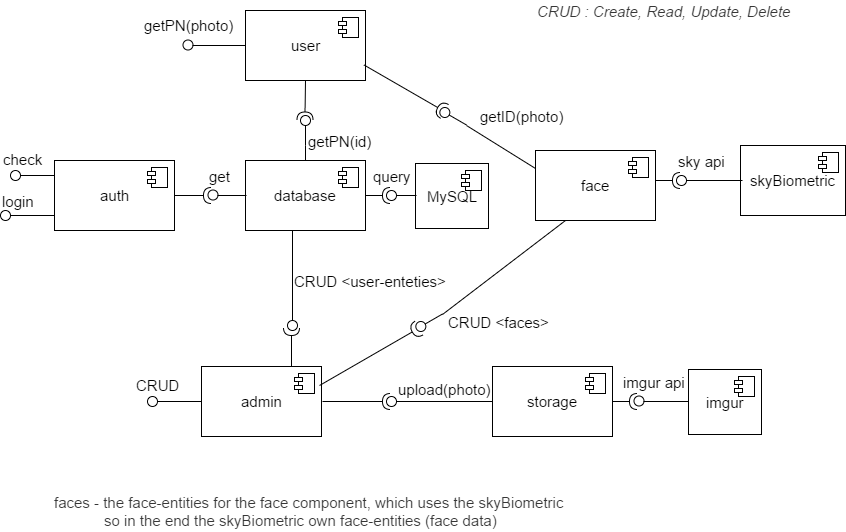
\includegraphics[width=150mm]{Architecture/ComponentDiagram.png}
	\caption{ComponentDiagram}
\end{figure}

\paragraph{Deployment Diagram}\label{deployment-diagram}

\begin{figure}[ht!]
	\centering
	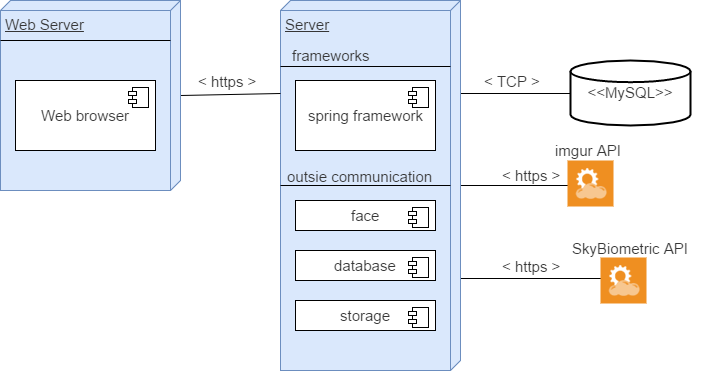
\includegraphics[width=150mm]{Architecture/DeploymentDiagram.png}
	\caption{DeploymentDiagram}
\end{figure}

\newpage
\section{Components - Design patterns and static modeling (Class Diagrams)}
This section describes the design patterns of each component(Database, Storage, Face, Admin, User and Authentication) of the system. In general, the system will be divided into Model-View-Controller(MVC) pattern where database, storage and face components represents the model; admin, user and authentication components represents the controller and the user who will use the API will be the view of the system (possibly inc. local view-controller). For the purpose of implementation, database, storage and face components will be embedded into one component called utils-service(these components will be independent of each other) whereas user and admin will be implemented separately; and authentication will be embedded into the main component called faceRecognition-service-api where all the components of the system will be integrated.
\newline

\noindent
Below sections will further describe the design patterns of each component as well as its class diagram:

\subparagraph{1. Database: }It is one of the most important component of the system because it contains the domain of the system as well as shared by all the controllers(user, admin and authentication). The biggest problem in this component is to encapsulate the functionality so that user and authentication component cannot use admin functionality and vice versa. To overcome this problem, Facade pattern will be used. This pattern will help in various ways such as database component will provide separate interfaces for each of the controller in order to get encapsulation; controllers will not get any extra information then needed; reduce the complexity of the component etc. Below diagram shows how database component provide three separate interfaces for the admin, user and authentication component.

\begin{figure}[ht!]
    \centering
	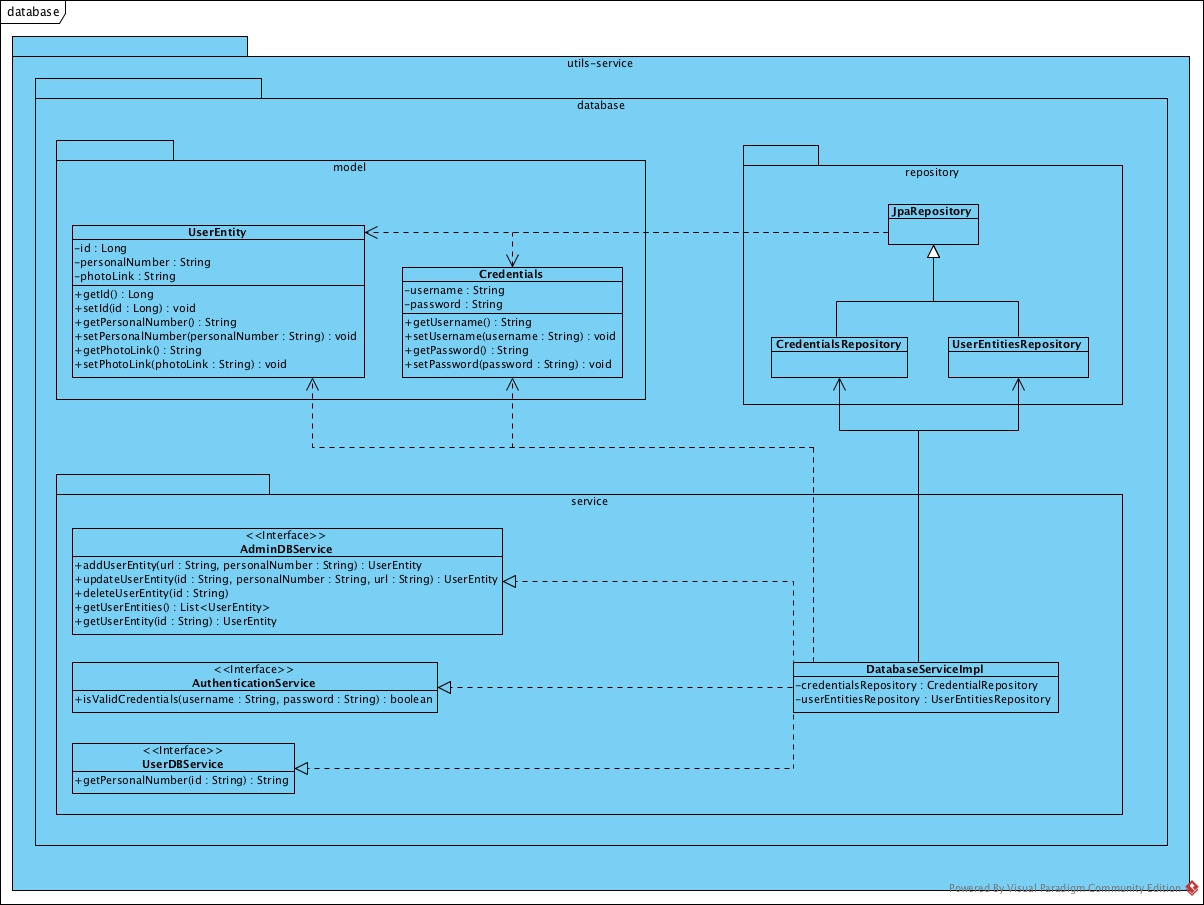
\includegraphics[width=130mm]{ClassDiagrams/new/database.jpg}
	\caption{Class diagram of database component}
\end{figure}

\newpage
\subparagraph{2. Storage: }This component is not as complex as database because only admin component will interact with it. This component will interact with one outer component called 'imgur' for saving the images into it. Like database component, Facade pattern is used to provide a simple and clear functionality to the admin component because admin component does not need to know how this component works. Below diagram shows how storage component provide nice and clear interfaces for the admin component.

\begin{figure}[ht!]
    \centering
	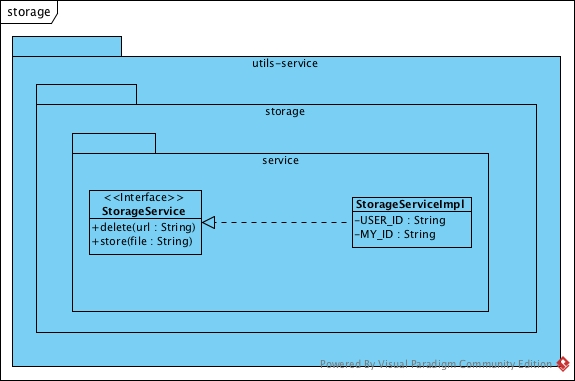
\includegraphics[width=110mm]{ClassDiagrams/new/storage.jpg}
	\caption{Class diagram of storage component}
\end{figure}

\subparagraph{3. Face: }This component is more complex than storage component due to encapsulation problem like database component because user and admin component will interact with it. In addition, it also interact with outer comoponent called 'SkyBiometry' for recognizing the faces. Like database component, it also use Facade pattern and below diagram shows how this component encapsulate the functionality by providing the seprate interfaces to admin and user component .

\begin{figure}[ht!]
    \centering
	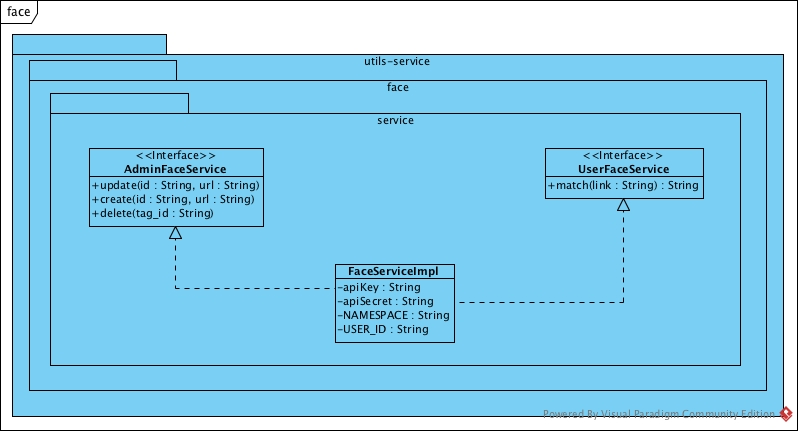
\includegraphics[width=125mm]{ClassDiagrams/new/face.jpg}
	\caption{Class diagram of face component}
\end{figure}

\newpage
\begin{figure}[ht!]
 \centering
    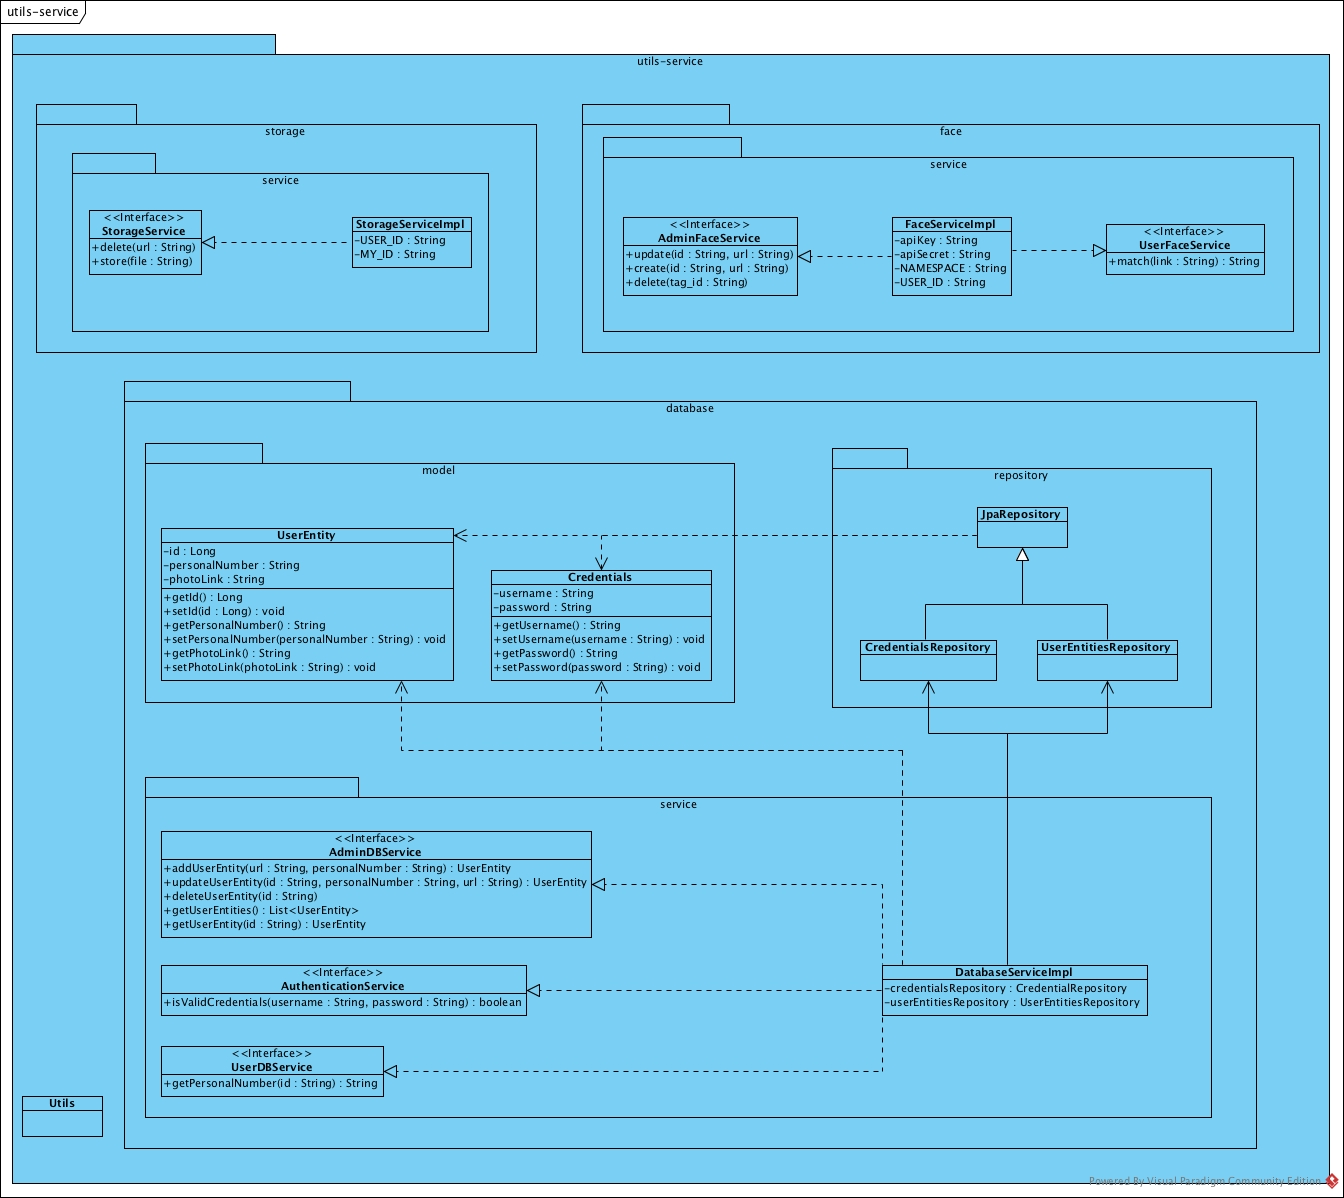
\includegraphics[width=170mm]{ClassDiagrams/new/utils-service.jpg}
    \caption{Overview of database, storage and face components embeeded inside the utils-service.
    \newline
    NOTE: 'Utils' class is for integration purpose and 'JpaRepository' is a part of spring framework.}
\end{figure}

\newpage
\subparagraph{4. Admin: }
This component use most of the important functionality of the system. However, it have no big problem related to the interaction with model because it simply use the interfaces provided by the database, face and storage component. The only problem is to encapsulate the data from view because it directly interact with the user API requests. Similarly, like other components, this component use same approach (Facade pattern) to encapsulate the data. It provide an interface to which the view will interact. This pattern helps to make the design more simple, flexible and reliable. Below diagram shows how this component encapsulate the data by providing interface to the controller which will interact with the view(user).

\begin{figure}[ht!]
    \centering
	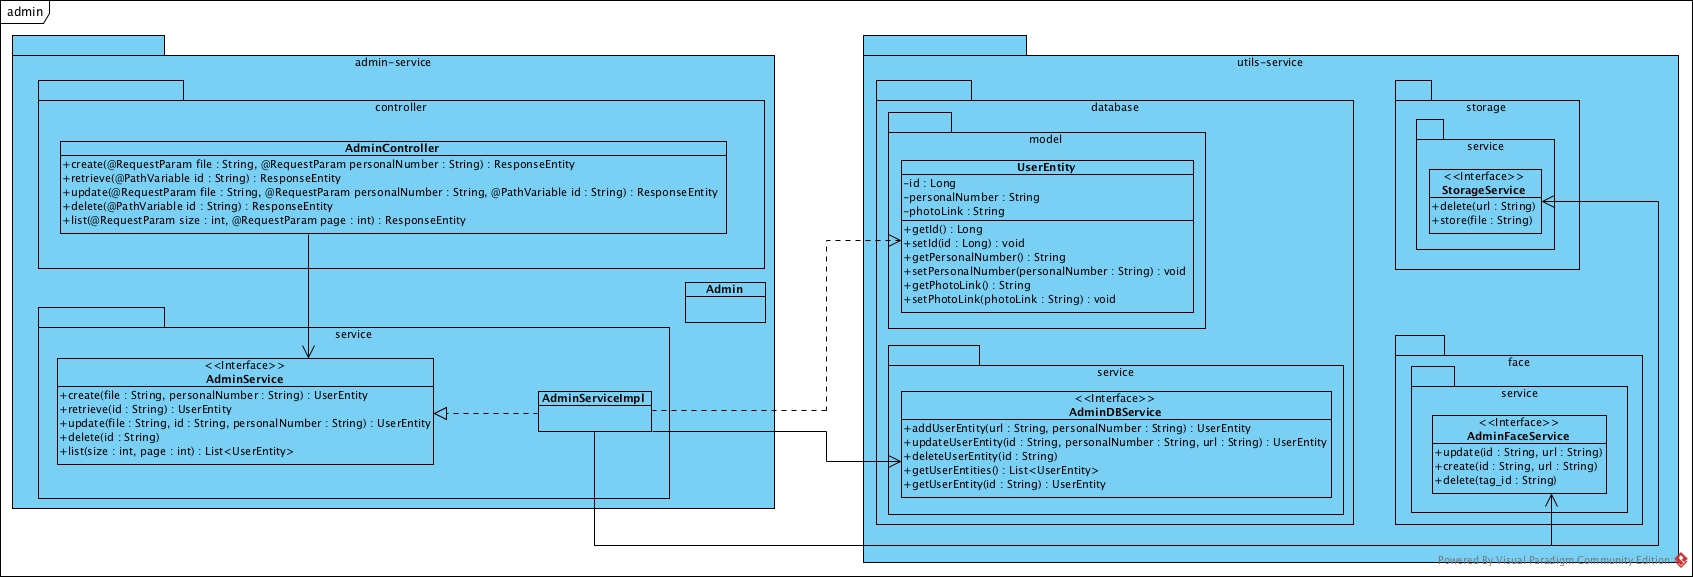
\includegraphics[width=150mm]{ClassDiagrams/new/admin.jpg}
	\caption{Class diagram of admin component}
\end{figure}

\subparagraph{5. User: }The structure and behaviour of this component is similar to admin component. Again, the only problem is to encapsulate the data from view and it use exactly the same approach as admin component in order to overcome the problem. Below diagram show how this component encapsulate the data from view by providing an interface to the controller.

\begin{figure}[ht!]
    \centering
	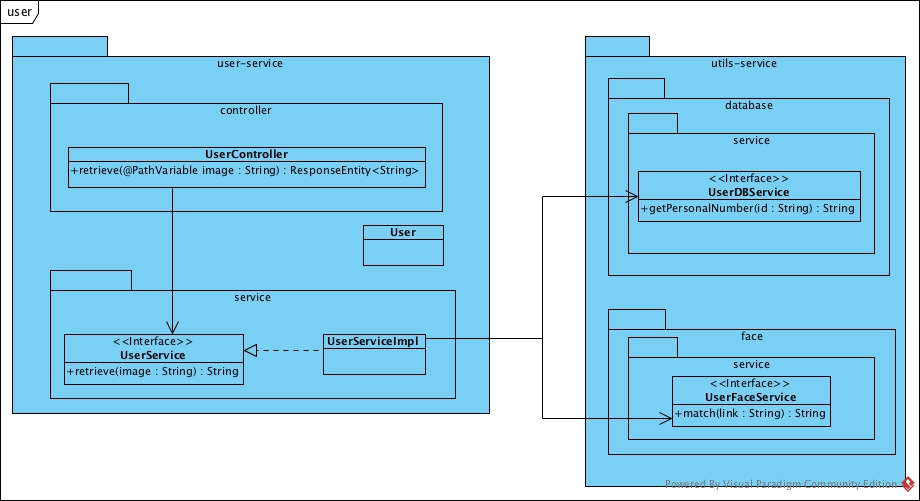
\includegraphics[width=130mm]{ClassDiagrams/new/user.jpg}
	\caption{Class diagram of user component}
\end{figure}

NOTE: 'Admin' and 'User' classes are  for integration purpose.


\newpage
\subparagraph{6. Authentication: } This component will be embedded into main component where all the other components will be integrated. This component will mostly use in built security functionality provided by spring framework for authenticating the user. However, for validating dynamic credentials(username and password), this component will use interface provided by database component. Below diagrams shows this component structure.

\begin{figure}[ht!]
    \centering
	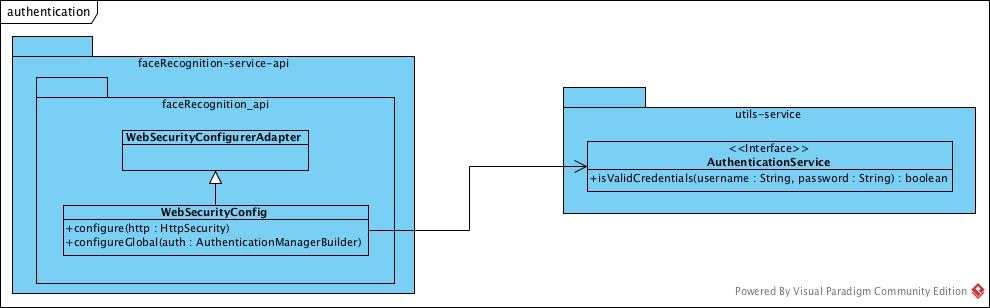
\includegraphics[width=130mm]{ClassDiagrams/new/authentication.jpg}
	\caption{Class diagram of authentication component}
\end{figure}

NOTE: 'WebSecurityConfigurerAdapter' and 'WebSecurityConfig' classes are part of spring data security framework.

\subparagraph{Integration: } For integrating all the components, we will use inbuild functionality provide by spring framework. Below diargram show the integration structure.

\begin{figure}[ht!]
    \centering
	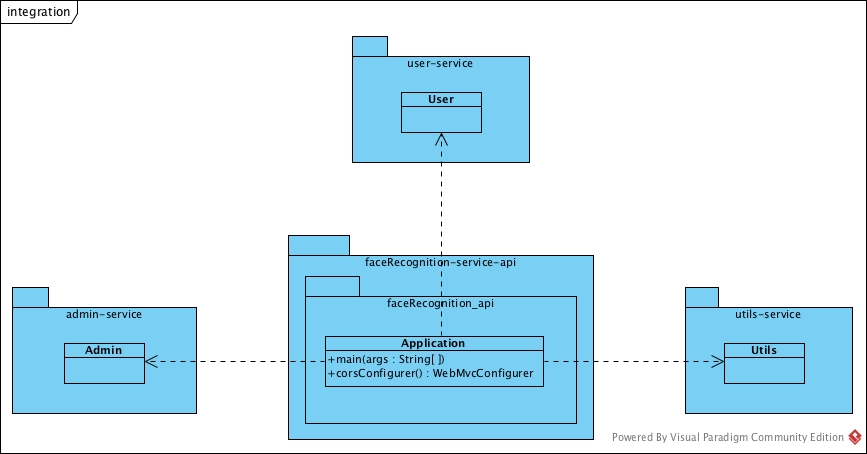
\includegraphics[width=130mm]{ClassDiagrams/new/integration.jpg}
		\caption{Class diagram of system integration}
\end{figure}

\newpage
\subparagraph{Complete System: } Below class diagram shows the complete system
		\centering
	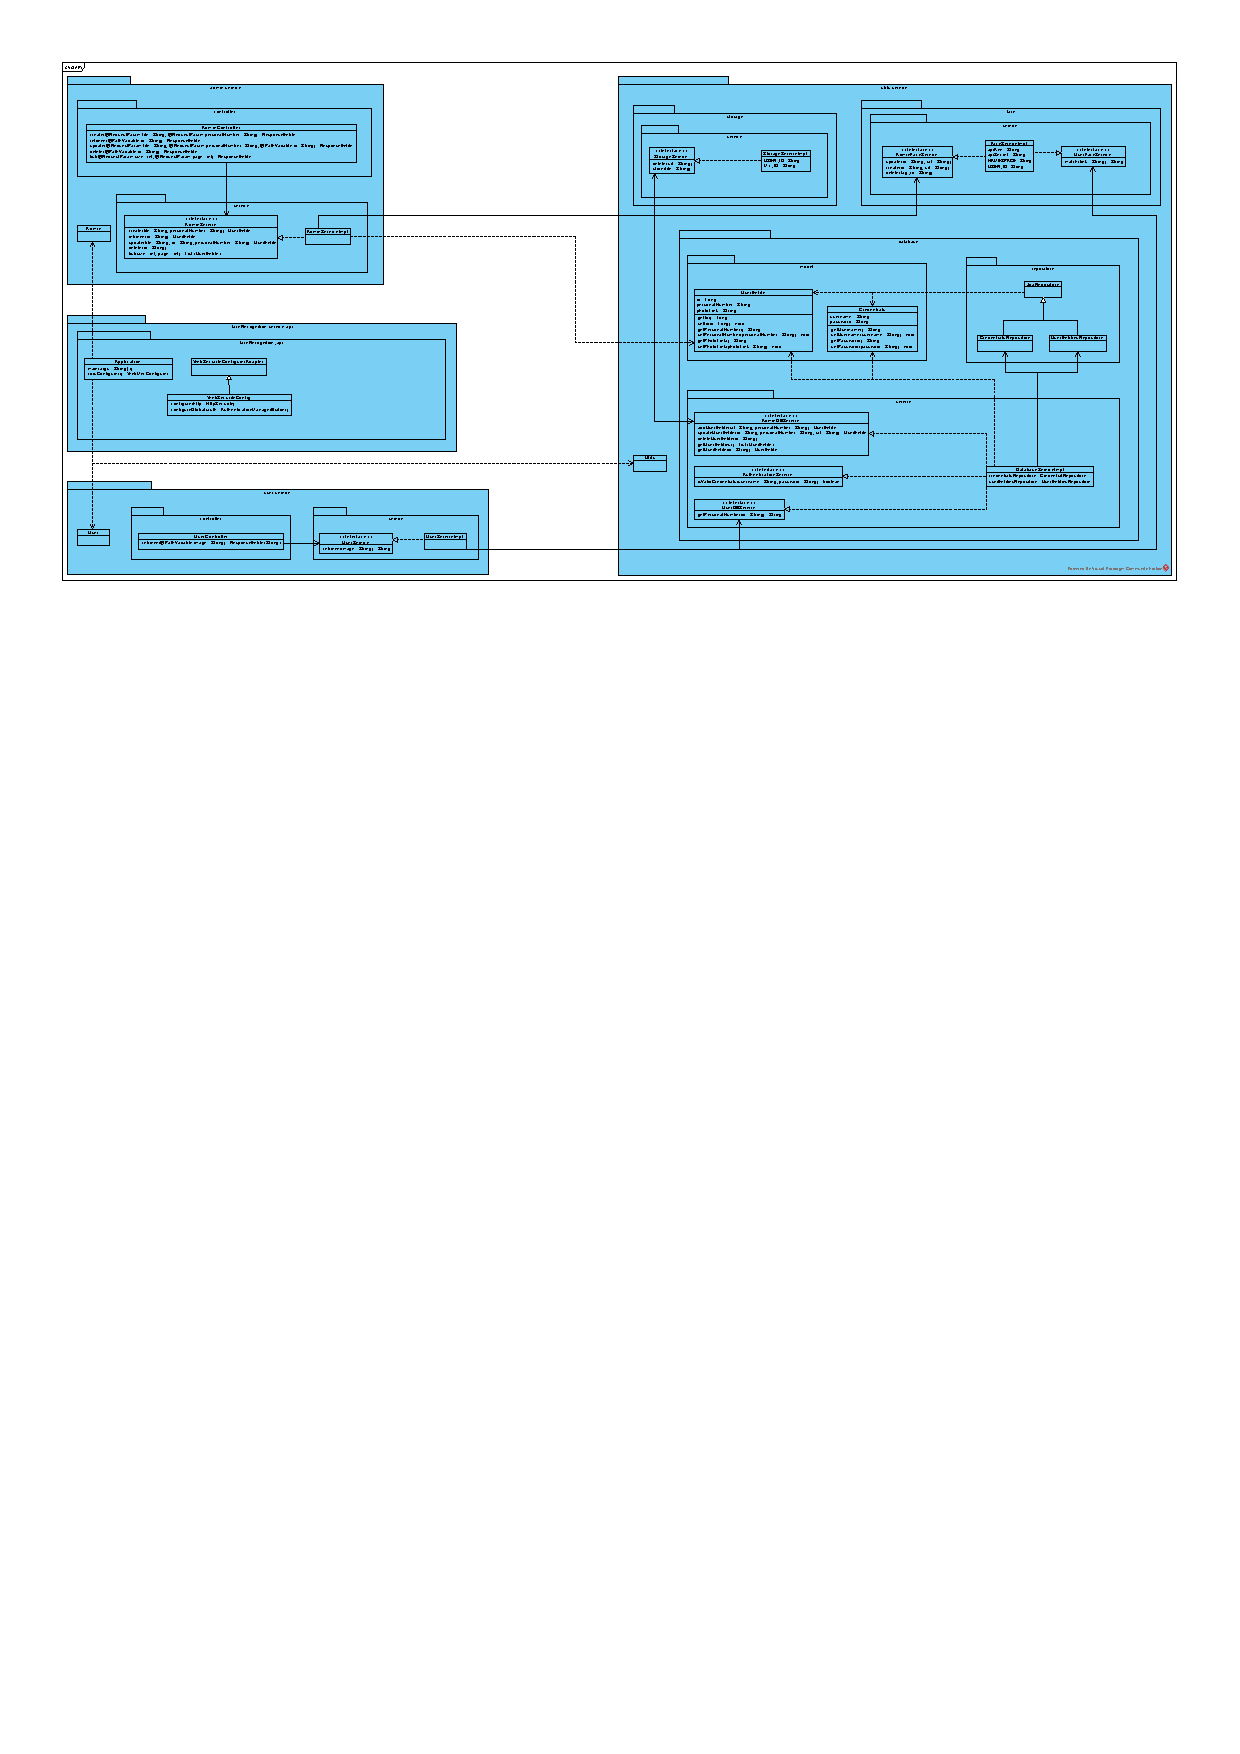
\includegraphics[scale=0.8]{ClassDiagrams/new/system.pdf}

\newpage
\section{Use cases - Behavioral modeling (Sequence Diagrams)}

\begin{figure}[ht!]
	\centering
	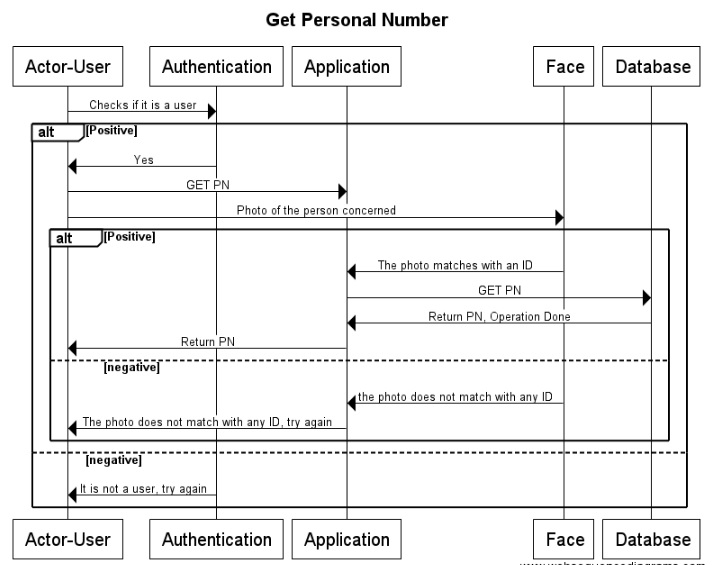
\includegraphics[width=150mm]{SequenceDiagrams/GetPN.jpg}
	\caption{Sequence diagram referred to "5.2 UAM: GET Personal Number" in the requirement document. \label{1}}
\end{figure}

\begin{figure}[ht!]
	\centering
	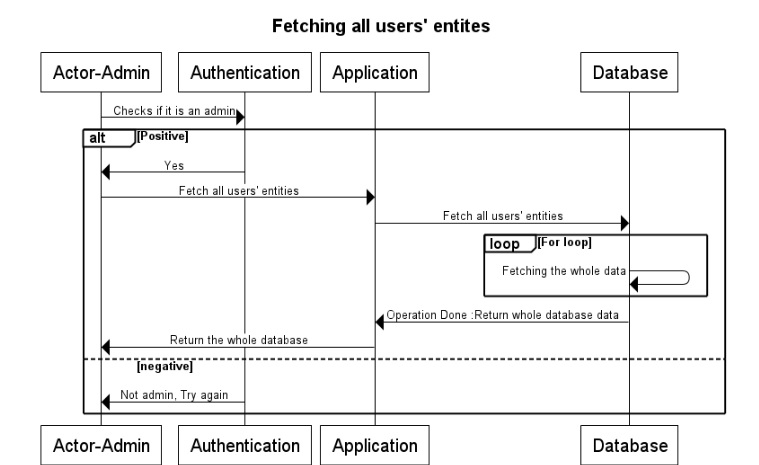
\includegraphics[width=150mm]{SequenceDiagrams/FetchAllUsers.jpg}
	\caption{Sequence diagram referred to "5.3 ARM: Get List of User-Entities" in the requirement document. \label{2}}
\end{figure}
\begin{figure}[ht!]
	\centering
	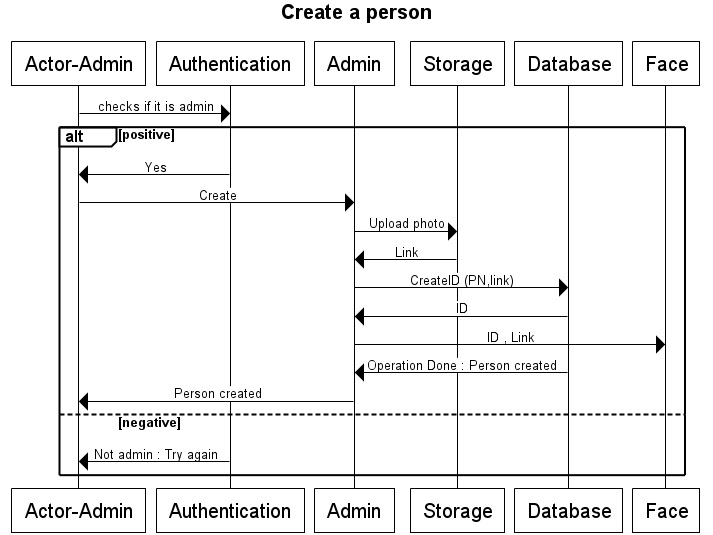
\includegraphics[width=150mm]{SequenceDiagrams/Create.jpg}
	\caption{Sequence diagram referred to "5.4 ARM: Add an User-Entity" in the requirement document. \label{3}}
\end{figure}

\begin{figure}[ht!]
	\centering
	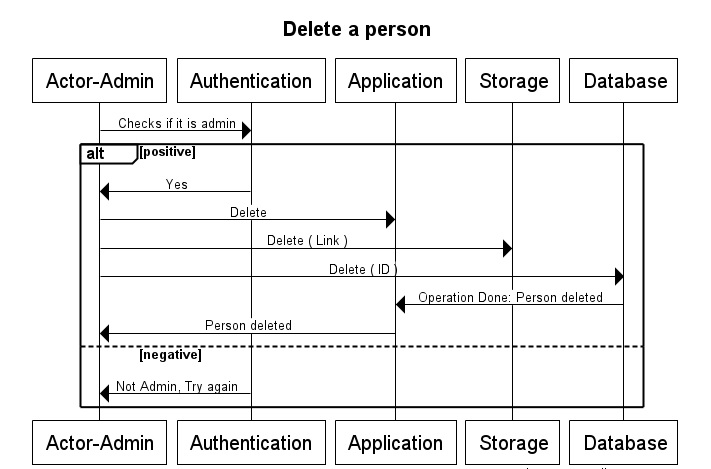
\includegraphics[width=150mm]{SequenceDiagrams/Delete.jpg}
	\caption{Sequence diagram referred to "5.5 ARM: Delete an User-Entity" in the requirement document. \label{4}}
\end{figure}

\begin{figure}[ht!]
	\centering
	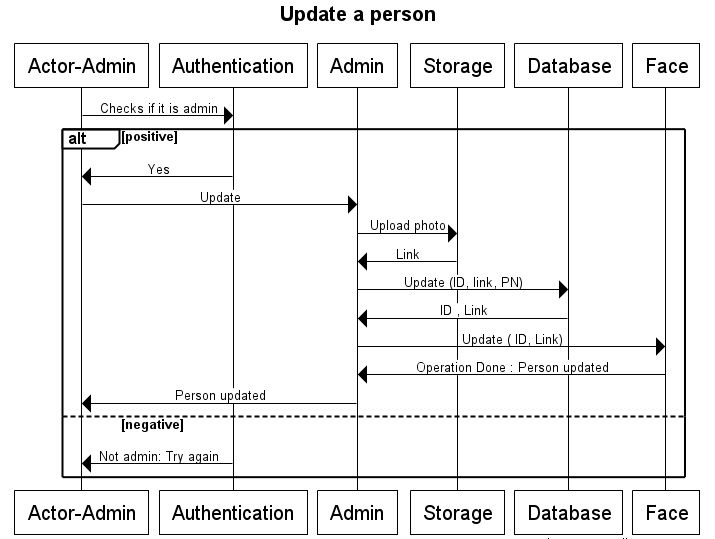
\includegraphics[width=150mm]{SequenceDiagrams/Update.jpg}
	\caption{Sequence diagram referred to "5.6 ARM: Update User-Entity" in the requirement document. \label{5}}
\end{figure}

\begin{figure}[ht!]
	\centering
	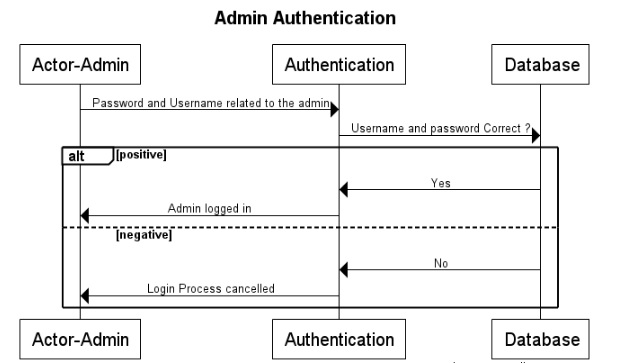
\includegraphics[width=150mm]{SequenceDiagrams/AdminAuth.jpg}
	\caption{Sequence diagram referred to "5.7 ARM: Authenticate Admin" in the requirement document. \label{6}}
\end{figure}
\begin{figure}[ht!]
	\centering
	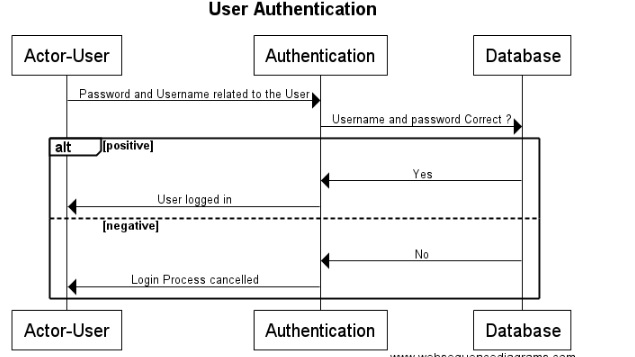
\includegraphics[width=150mm]{SequenceDiagrams/UserAuth.jpg}
	\caption{Sequence diagram referred to "5.8 URM: Authenticate User" in the requirement document. \label{7}}
\end{figure}
\end{document}